\subsection{Der \emph{Spawner}}

Das zentrale Element der Zugerzeugung ist die Klasse \code{Spawner}. Die Architektur aller an der Zeugerzeugung beteiligten Klassen ist in \autoref{fig:spawner-class} dargestellt. Die Klasse \code{Spawner} erbt, wie die anderen zentralen Klassen des Systems, von der Klasse \code{Component} und erhält damit Zugriff auf den \code{EventBus}, welcher in einem folgenden Abschnitt beschrieben wird, und auf die Methode \code{next\_tick}. Diese Methode wird in jedem Zeitintervall der Simulation einmal aufgerufen und gibt der Komponente die Möglichkeit, auf die Simulation zu reagieren. Weiterhin realisiert die Klasse \code{Spawner} die \code{ISpawnerDisruptor}-Schnittstelle, welche eine Fehlerinjektion \cite{persitzky_fehlerinjektion_2023} ermöglicht. Der \code{Spawner} besitzt die Attribute \code{configuration}, welches im folgenden Abschnitt näher beleuchtet wird, und \code{schedules}, bei dem es sich um eine Liste Abfahrtsplänen (\code{Schedule}-Objekte) handelt.

\begin{figure}[!ht]
	\centering
	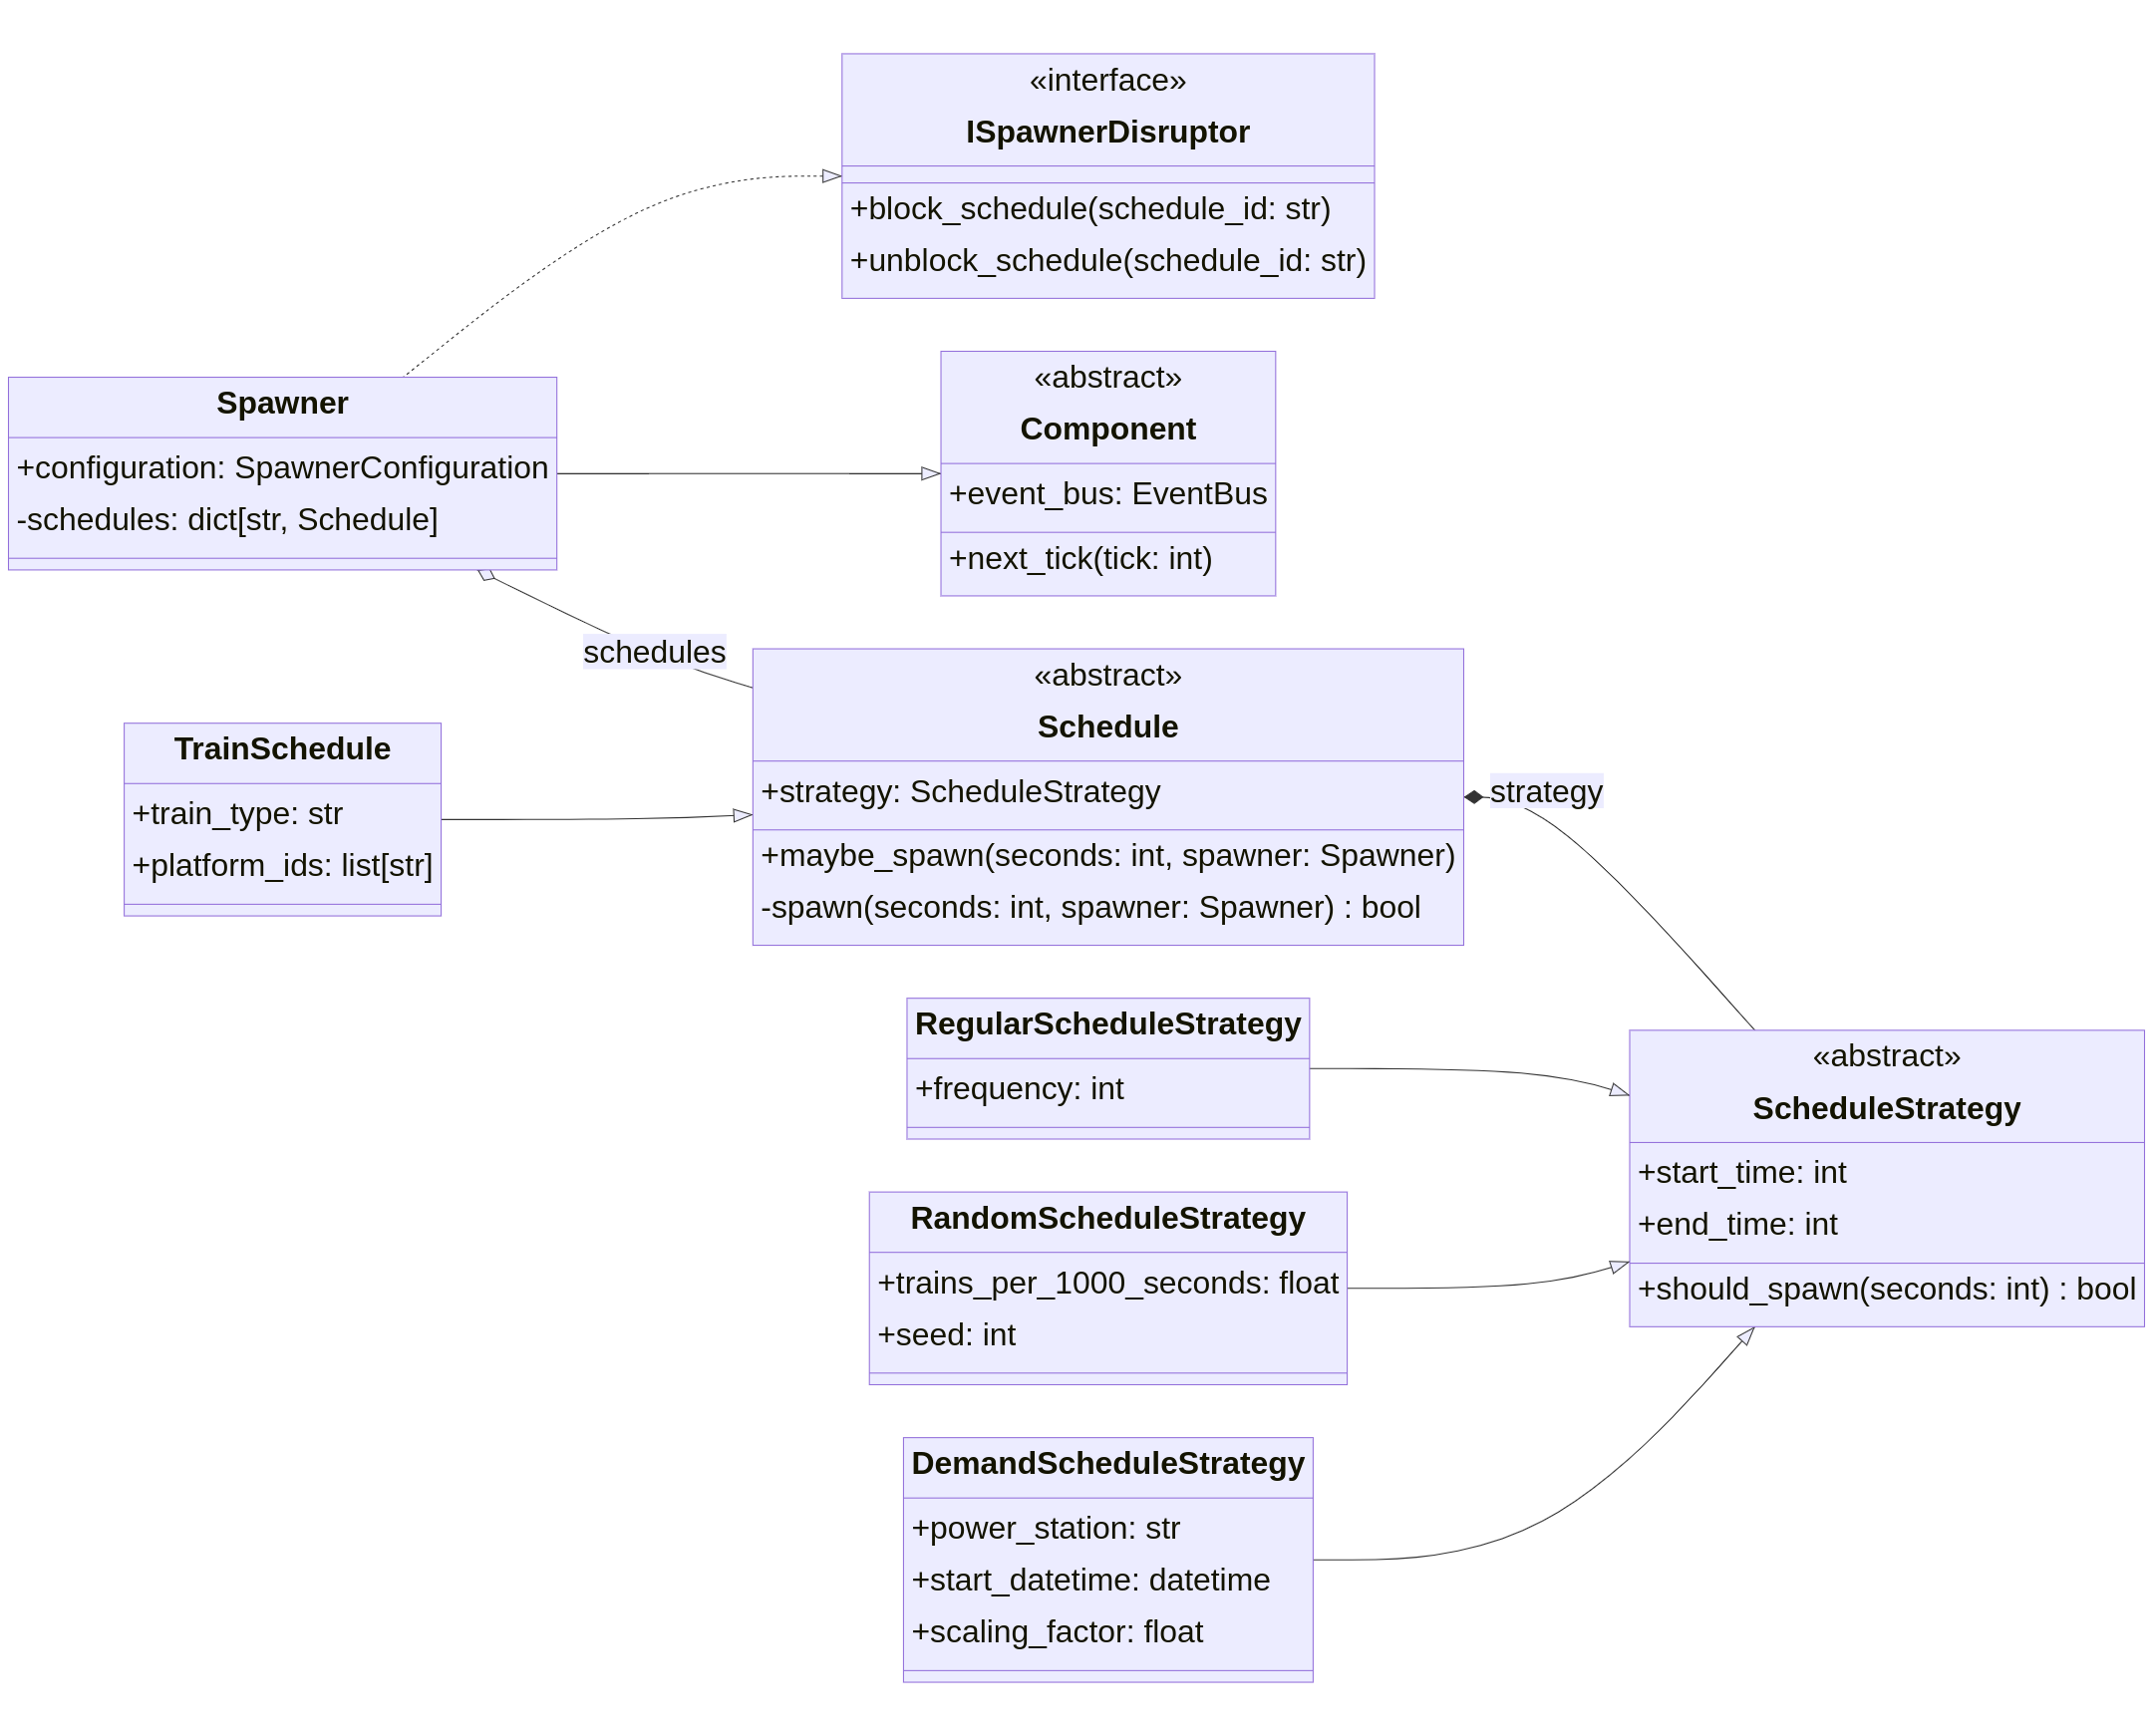
\includegraphics[width=1.0\linewidth]{images/diagrams/spawner-class.png}
	\caption{Klassendiagramm der Zugerzeugung}
	\label{fig:spawner-class}
\end{figure}

Die Klasse \code{Schedule} ist abstrakt und bietet damit die Möglichkeit der Spezialisierung. Die einzige bisher implementierte Spezialisierung ist der \code{TrainSchedule}, welcher speziell für die Erzeugung von Zügen verantwortlich ist. Wir haben uns für eine abstrakte \code{Schedule}-Klasse entschieden, um die Möglichkeit zu haben, das System in Zukunft um Abfahrtspläne anderer Verkehrsteilnehmer zu erweitern. Denkbar wäre bspw. die Simulation von Fußgängern, die gleichzeitig als Passagiere für Personenzüge fungieren. Diese Funktionalität könnte in einer Klasse \code{PedestrianSchedule} implementiert werden, welche ebenfalls von \code{Schedule} erbt. Eine Instanz eines \code{TrainSchedule} Attribute, welche den Zugtyp (\code{train\_type}) und die Liste der anzufahrenden Haltestellen (\code{platform\_ids}) enthalten.\\
\\
Um eine zukünftige Erweiterbarkeit zu gewährleisten, wurde die Klasse \code{Schedule} so implementiert, dass der Algorithmus, welcher die Abfahrzeiten bestimmt, von der eigentlichen \code{Schedule}-Klasse unabhängig ist. Ein \code{Schedule}-Objekt hält eine Referenz auf ein \code{ScheduleStrategy}-Objekt, welches einen Algorithmus zur Bestimmung der Abfahrtszeiten implementiert. Diese Klasse stellt eine Start- und eine Endzeit (\code{start\_time} und \code{end\_time}) bereit, welche die Zeitspanne festlegen, in der die Abfahrtszeiten bestimmt werden. Mit der Methode \code{should\_spawn} kann für eine bestimmte Zeit abgefragt werden, ob ein Zug zu erzeugen ist. Von der abtrakten Klasse \code{ScheduleStrategy} erben die Klassen \code{RegularScheduleStrategy}, \code{RandomScheduleStrategy} und \code{DemandScheduleStrategy}, welche das Verhalten der drei zuvor beschriebenen Abfahrtspläne implementieren.\\
\\
Die Klasse \code{RegularScheduleStrategy} implementiert die regulären Abfahrtspläne und besitzt das Attribut \code{frequency}, welches die Häufigkeit der regelmäßig abfahrenden Züge angibt. Die \code{RandomScheduleStrategy}-Klasse ist für die randomisierten Abfahrtspläne zuständig und besitzt dafür die Attribute \code{trains\_per\_1000\_seconds} und \code{seed}, welche die Wahrscheinlichkeit einer Abfahrt und einen Startwert für den Zufallszahlengenerator beinhalten. Letzteres Attribut dient der Reproduzierbarkeit von Simulationsergebnissen. Die \code{DemandScheduleStrategy}-Klasse implementiert die Abfahrtspläne, welche auf dem Kohlebedarf basieren. Die hält die Attribute \code{power\_station} für das betrachtete Kraftwerk, \code{start\_datetime} für das Startdatum der historischen Datenbasis und \code{scaling\_factor}, womit der Kohlebedarf skaliert werden kann, um bspw. eine unvollständige Auslastung eines Kraftwerks zu simulieren.

\autoref{fig:spawner-seq} zeigt das Verhalten der Zugerzeugung innerhalb eines Zeitintervalls der Simulation. Ein \code{Communicator}-Objekt\footnote{beschrieben in der Arbeit von \citeauthor{kamp_architektur_2023} \cite{kamp_architektur_2023}} sendet \code{next\_tick} an das \code{Spawner}-Objekt (1). Dieser sendet daraufhin \code{maybe\_spawn} an jedes Element in der Liste \code{schedules} und übergibt sich dabei selbst (2). Durch Aufruf von \code{should\_spawn} wird überprüft, ob ein Zug zu erzeugen ist (3). Ist dies der Fall, ruft das \code{Schedule}-Objekt auf sich selbst \code{spawn} auf (5), was dazu führt, dass \code{spawn\_train} an die übergebene \code{Spawner}-Instanz gesendet wird (6). Dort wird letztendlich die Schnittstelle zu \emph{SUMO} angesprochen, um einen Zug in die Simulation zu setzen.

\begin{figure}[!ht]
	\centering
	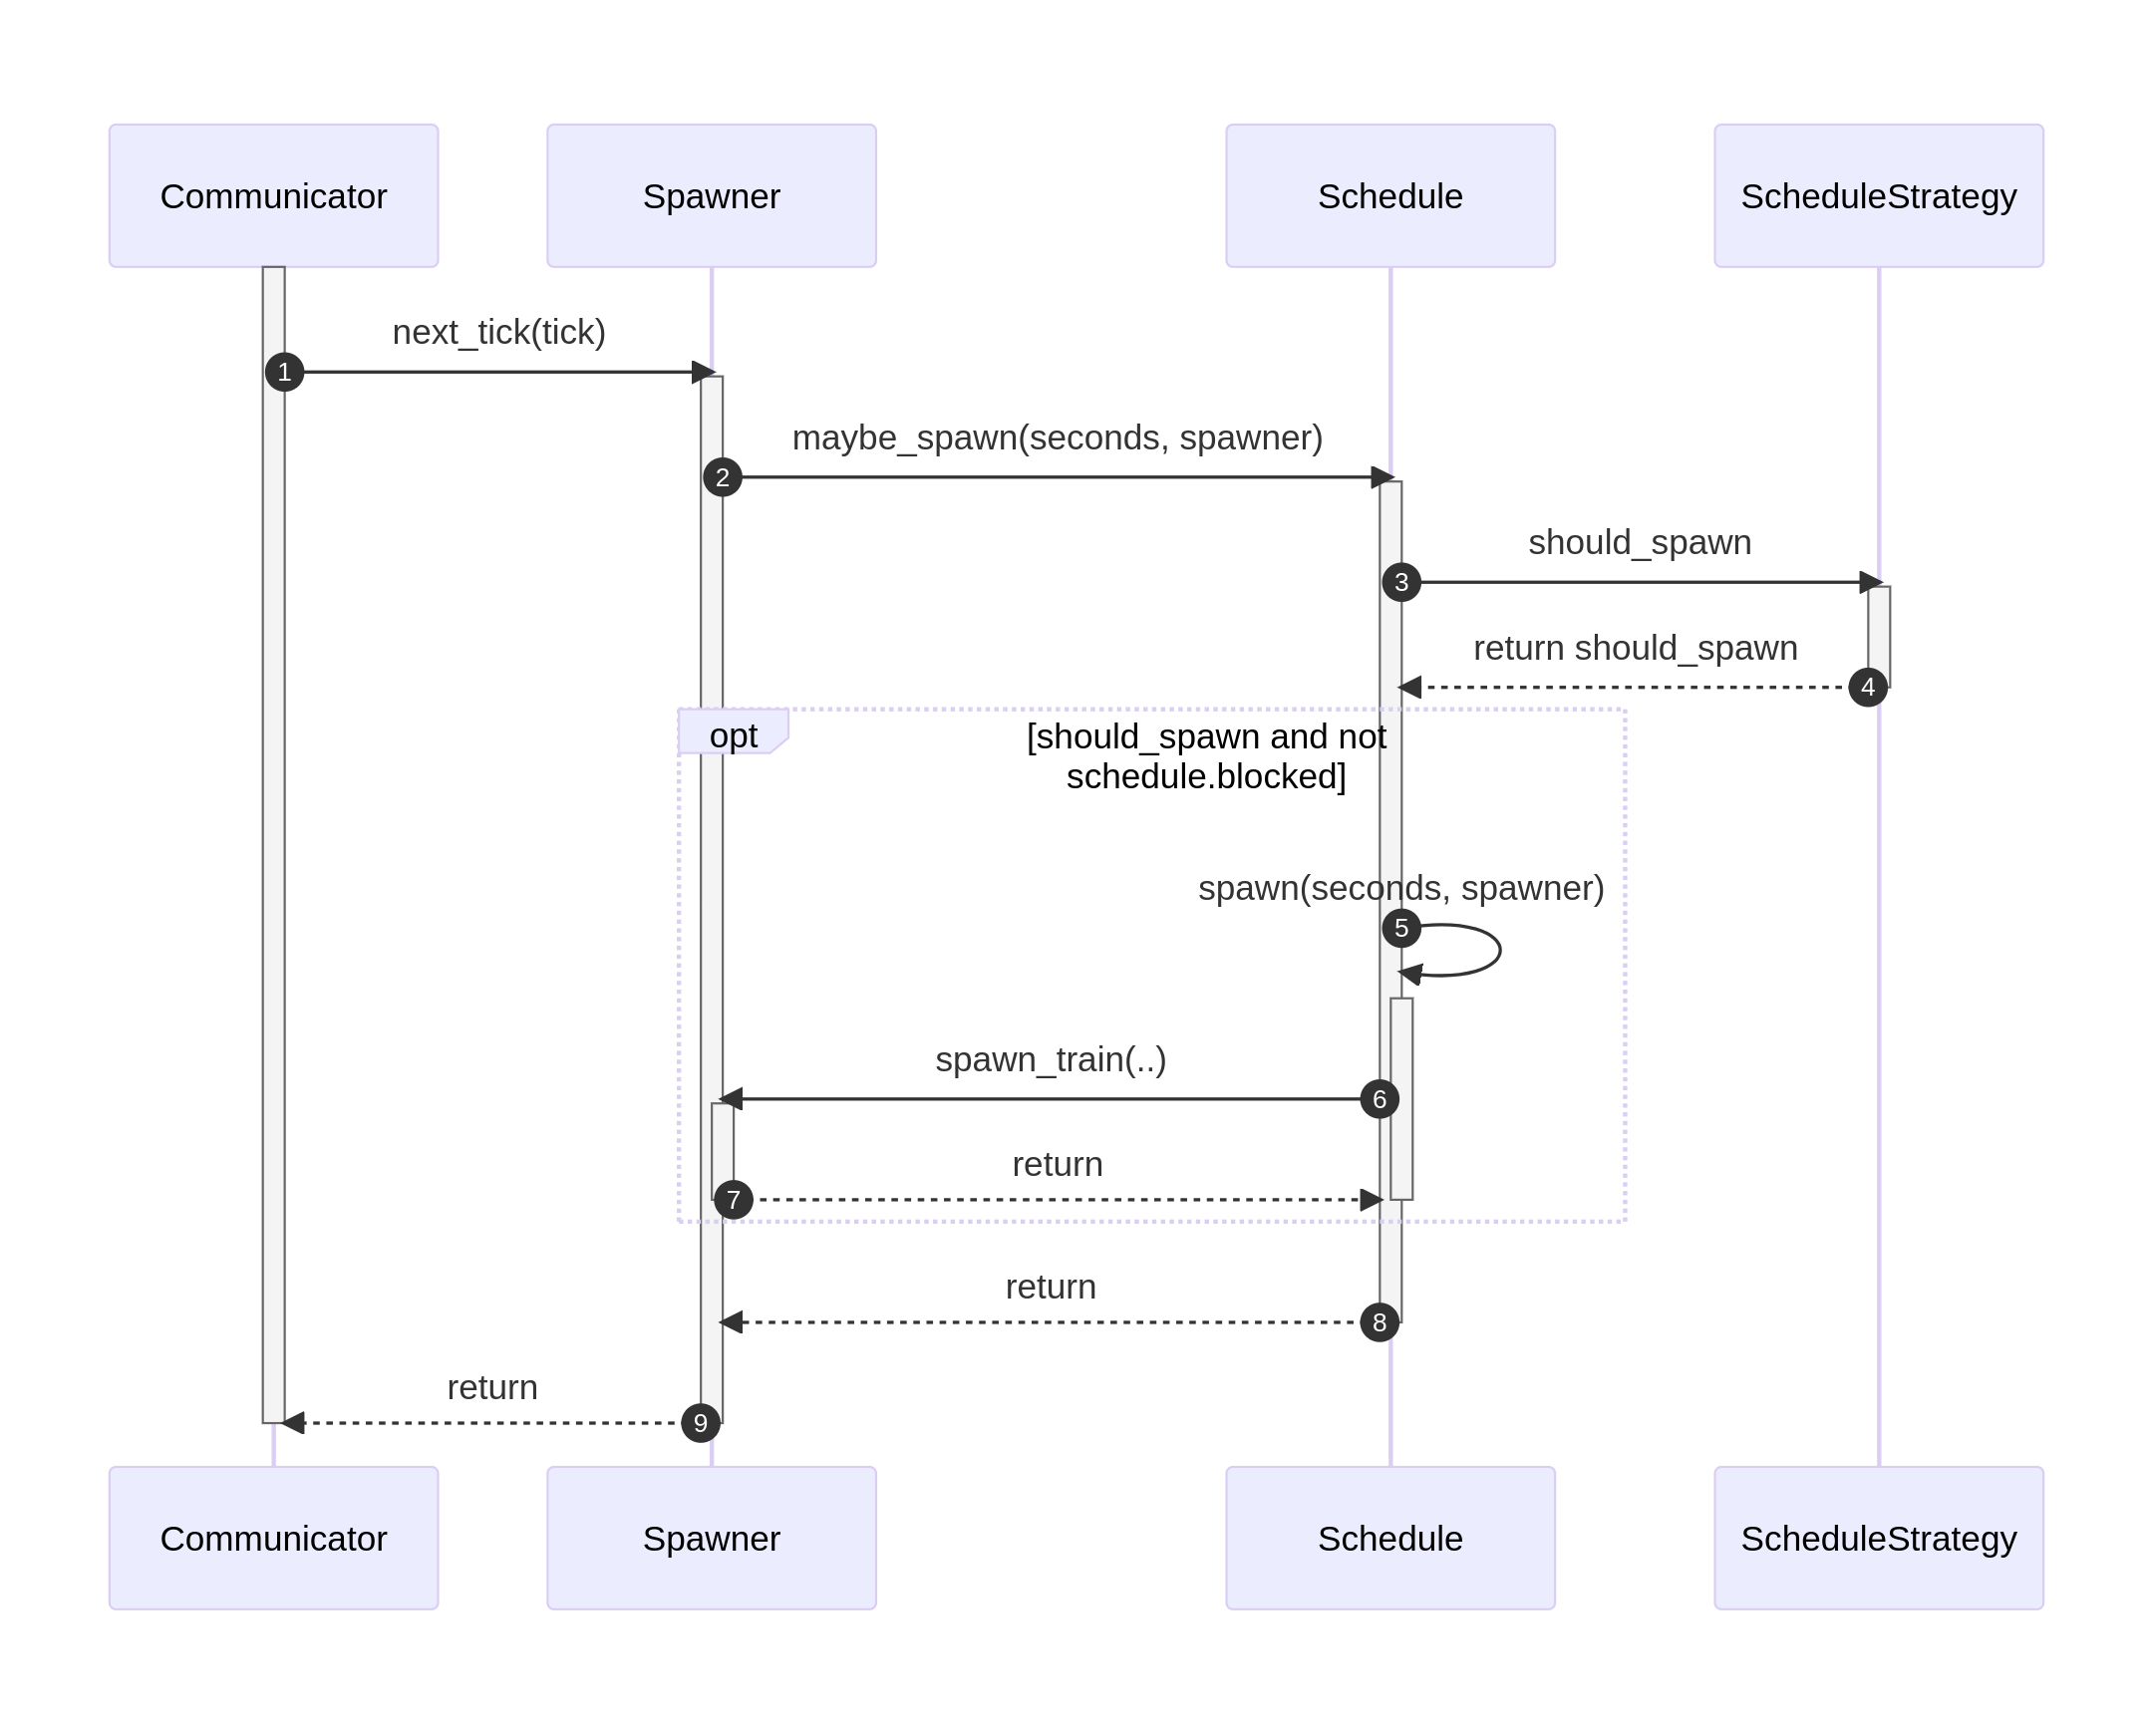
\includegraphics[width=1.0\linewidth]{images/diagrams/spawner-seq.png}
	\caption{Sequenzdiagramm der Zugerzeugung}
	\label{fig:spawner-seq}
\end{figure}

Bei diesem Mechanismus finden zwei Entwurfsmuster Anwendung. Der \code{Spawner} fungiert and \emph{Visitor} und besucht jedes Element in der Liste von \code{Schedule}-Objekten. Über einen \emph{Double-Dispatch} mit den Methoden \code{maybe\_spawn} und \code{spawn\_train} wird dabei erreicht, dass die Verantwortlichkeit der Implementierung zur Erzeugung von Zügen (und zukünftig evtl. weiterer Verkehrsteilnehmer) bei der Klasse \code{Spawner} liegt. Die Entscheidung hingegen wird von den \code{Schedule}-Objekten getroffen. Dadurch lassen sich in Zukunft relativ einfach weitere Arten von \code{Schedule}-Klassen hinzufügen. Die Klasse \code{Spawner} muss dazu nur um jeweils eine weitere Methode erweitert werden. Bei der Methode \code{maybe\_spawn} handelt es sich weiterhin um eine im abstrakten \code{Schedule} implementierte \emph{Template-Method}. Sie gibt den Ablauf der Entscheidung über die Zugerzeugug vor. Die konkreten Implementierungen für \code{spawn} und \code{should\_spawn} liegen jedoch in den konkreten Subklassen von \code{Schedule}  bzw. \code{ScheduleStrategy}. Auch hier ist der Vorteil, dass sich neue Algorithmen zur Bestimmung der Abfahrtszeiten relativ einfach hinzufügen lassen, ohne dass die Klasse \code{Spawner} angepasst werden muss.
